\documentclass[conference]{IEEEtran}
\usepackage[
    style=numeric,
    sorting=none
]{biblatex}
\usepackage{amsfonts}
\usepackage{amsmath}
\usepackage{booktabs, multirow}
\usepackage[dvipsnames]{xcolor}
\usepackage{tikz}
\usetikzlibrary{positioning,fit,backgrounds,scopes,decorations.pathreplacing,shapes.geometric}
\newcommand{\bibliofont}{\footnotesize}
\renewcommand\IEEEkeywordsname{Keywords}
\renewcommand\arraystretch{1.5}

\addbibresource{paper.bib}

\begin{document}

\author{
    \IEEEauthorblockN{{\bf German Arutyunov}\IEEEauthorrefmark{1}\\ \tt\footnotesize gaarutyunov@edu.hse.ru} \and
    \IEEEauthorblockN{{\bf Sergey Avdoshin}\IEEEauthorrefmark{1}\\ \tt\footnotesize savdoshin@hse.ru}
    \and
    \IEEEauthorblockA{\IEEEauthorrefmark{1}HSE University, 20, Myasnitskaya st., Moscow, Russia}
}

\title{GraphTyper: Neural Types Inference from Code Represented as Graph}

\begin{abstract}
    Although software development is mostly a creative process, there are many scrutiny tasks.
    As in other industries, there is a trend for automation of routine work.
    In many cases, machine learning and neural networks have become a useful assistant in that matter.
    Programming is not an exception:
    GitHub has stated that Copilot is already used to write up to 30\% of code in the company.
    Copilot is based on Codex, a Transformer model trained on code as a sequence.
    However, a sequence is not a perfect representation for programming languages.
    In this work, we claim and demonstrate that by combining the advantages of Transformers
    and graph representations of code, it is possible to achieve excellent results even with comparably small models.
\end{abstract}

\begin{IEEEkeywords}
    Neural networks, Transformers, graphs, abstract syntax tree
\end{IEEEkeywords}

\maketitle

\section{Introduction}\label{sec:introduction}
Application of Transformers yet again has managed to break the deadlock: this time in the task of code generation~\cite{hendrycks_measuring_2021,chen_evaluating_2021,li_competition-level_nodate,nijkamp_conversational_2022}.
Nevertheless, the versatile Transformer architecture has displayed good results on several benchmarks,
in the recent work~\cite{xu_systematic_2022} it was shown that increasing the size of the model doesn't result in a better performance.
Moreover, it is evident that context matters a lot to produce a working code.
However, it is not feasible to relentlessly increase the length of context sequence in a Transformer.
Therefore, a different approach is needed to boost the efficiency in the task of code synthesis~\cite{arutyunov_big_2022}.

First of all, an expressive code representation has to be selected.
Several ways including token-based, structured and graph-based approaches have been reviewed~\cite{sm_avdoshin_code_2022}.
For instance, graph representation using abstract syntax tree (AST), data-flow graph (DFG) and control-flow graph (CFG)
yield good results in such tasks as variable misuse detection and correction~\cite{allamanis_learning_2017}.
Such graph representation can capture an extensive amount of information about the programs code.

Secondly, a versatile model architecture that supports learning on graphs must be used.
Multiple models such as RNN~\cite{white_deep_2016}, LSTM~\cite{wei_supervised_2017} and CNN~\cite{mou_convolutional_2016} with flattened graphs have been used.
However, graph-aware model architecture is more suitable for the graph representation of code.
For this reason, Graph Neural Networks (GNN) are a more reasonable choice of architecture,
namely message-passing neural networks~\cite{allamanis_learning_2017}.

Nonetheless, in this work we aim to make the most from both: the advantages of Transformer architecture and graph representation of code.
For instance, we will use Transformer architecture optimizations~\cite{choromanski_rethinking_2020} and graph code representation created from AST.
To make this possible we will use Pure Transformers~\cite{kim_pure_2022} instead of models that have some architectural alterations to support graph structure~\cite{kreuzer_rethinking_2021,dwivedi_generalization_2021,ying_transformers_2021}.

\section{Problem Statement}\label{sec:problem-statement}
In this work, we test the ability of Pure Transformers to add types to Python source code based on its graph structure.
This task was selected as a starting point for future research due to its practical relevance.

Firstly, dynamically typed languages, such as Python and JavaScript, have gained quite some traction during the last years~\cite{kaggle-survey-2021}.
However, it doesn't mean they're easier~\cite{robillard2009what, robillard2011afield, zibran2011useful} or less error-prone than statically typed languages~\cite{alzahrani2018pythonvscplus}.
Moreover, lack of type hints in libraries might lead to expensive errors in fields such as Data Science~\cite{reimann2023safeds}.

There are some tools outside the neural networks domain that perform static type checking and inferencing type annotations~\cite{pyre, PyType}.
Nonetheless, these utilities do not work without type hints in the source code of the dependencies, which is pretty common.
To alleviate this, there are proposals about Domain-Specific Languages (DSL) for Data Science~\cite{reimann2023safeds}.
However, it wouldn't work on existing code base and massive adoption is not very likely.

On the other hand, absence of type hints is not a restriction for neural networks
(see. Section~\ref{subsec:using-the-model-without-node-type-annotations}).
In addition, they don't only find erroneous types in existing codebase~\cite{allamanis2020typilus}
but can also be used during development to annotate code on the fly~\cite{mir_type4py_2021}.

Most importantly, inferring types requires a model to learn a lot about the source code.
Therefore, developing a model with versatile architecture to infer types allows it to be later applied for other tasks.

\subsection{Metrics}\label{subsec:metrics}

To test the model, we use two metrics from the Typilus paper~\cite{allamanis2020typilus}:

\begin{description}
    \item{Exact Match: Predicted and ground truth types match exactly.}
    \item{Match up to Parametric Type: Exact match when ignoring all type parameters.}
\end{description}

\section{Previous Work}\label{sec:previous-work}
\subsection{Graph Representation of Code}\label{subsec:graph-representation-of-code}

AST and DFG have already been used with Transformers in the code generation and summarization tasks~\cite{wang_unified_2022,tang_ast-transformer_2021,sun_treegen_2020}.
In addition, some joint graph structure representations that include different code graphs have been developed,
namely code property graph (CPG)~\cite{yamaguchi2014modeling}, that incorporates AST, CFG and PDG (program dependency graph).
This graph representation has already been used for vulnerability detection~\cite{yamaguchi2014modeling} and similarity detection~\cite{liu2023learning}.

\subsection{Graph Transformers}\label{subsec:graph-transformers}

Graph Transformers is a novel architecture that has been developing in the past few years.
They have been applied for several tasks, mostly in the field of molecule generation, node classification and node feature regression~\cite{kim_pure_2022,kreuzer_rethinking_2021,dwivedi_generalization_2021,ying_transformers_2021}.
Apart from models with alterations to Transformer base architecture~\cite{ying_transformers_2021, kreuzer_rethinking_2021}
researchers have recently developed simpler models~\cite{kim_pure_2022} that are compatible with many popular techniques developed for
standard Transformers~\cite{choromanski_rethinking_2020}.

\subsection{Type Inference with Neural Networks}\label{subsec:type-inference-with-neural-networks}

The task of type inference has been also extensively covered in recent research.
Many different architectures have been used for this task: GNNs~\cite{allamanis2020typilus}, RNNs~\cite{pradel2020typewriter, mir_type4py_2021} and Transformers~\cite{jesse2021typebert, peng2023generative} among others.
Moreover, graph representation of code has been used for the task of type inference in dynamically typed programming languages such as Python~\cite{allamanis2020typilus} and Javascript~\cite{schrouff_inferring_2019}.

However, the power of Graph Transformers and Graph Representation of code hasn't been combined yet to solve the task of
type inference in source code.
This is the gap our model aims to fill.
The results of our model compared to previous work~\cite{mir_type4py_2021, allamanis2020typilus, pradel2020typewriter, jesse2021typebert, peng2023generative} are displayed in Table~\ref{tab:results}.

\begin{table}
    \centering
    \caption{Quantitative evaluation of models measuring their ability to
    predict ground truth type annotations.}
    \label{tab:results}
    \begin{tabular}{llrr}
\toprule
 &  & Exact Match & Up to Parametric Type \\
Top-n & Model &  &  \\
\midrule
\multirow[c]{6}{*}{Top-1} & GraphTyper & 34.71 & 36.43 \\
 & TypeBERT & 45.40 & 48.10 \\
 & Typilus & 56.10 & 58.30 \\
 & Type4Py & 66.10 & 74.20 \\
 & TypeWriter & 75.80 & 80.60 \\
 & TypeGen & \bfseries 79.20 & \bfseries 87.30 \\
\cline{1-4}
\multirow[c]{6}{*}{Top-3} & GraphTyper & 45.47 & 55.02 \\
 & TypeBERT & 51.40 & 53.50 \\
 & Typilus & 63.70 & 67.30 \\
 & Type4Py & 71.60 & 79.80 \\
 & TypeWriter & 78.10 & 83.80 \\
 & TypeGen & \bfseries 85.60 & \bfseries 91.00 \\
\cline{1-4}
\multirow[c]{6}{*}{Top-5} & GraphTyper & 50.70 & 64.58 \\
 & TypeBERT & 54.10 & 56.50 \\
 & Typilus & 65.90 & 70.40 \\
 & Type4Py & 72.70 & 80.90 \\
 & TypeWriter & 78.70 & 84.70 \\
 & TypeGen & \bfseries 87.00 & \bfseries 91.70 \\
\cline{1-4}
\bottomrule
\end{tabular}


\end{table}

\section{Proposed Solution}\label{sec:proposed-solution}
\subsection{Dataset}\label{subsec:dataset}

To train and test the model we gathered 600 Python repositories from GitHub containing type annotations from Typilus~\cite{allamanis2020typilus}.
We clone these repositories and utilize pytype for static analysis, augmenting the corpus with inferred type annotations.
The top 175 most downloaded libraries are added to the Python environment for type inference.
Through deduplication, we remove over 133,000 near code duplicates to prevent bias.

The resulting dataset comprises 118,440 files with 5,997,459 symbols, of which 252,470 have non-Any non-None type annotations.
The annotations exhibit diversity with a heavy-tailed distribution, where the top 10 types cover half of the dataset, primarily including str, bool, and int.
Only 158 types have over 100 annotations, while the majority of types are used fewer than 100 times each, forming 32\% of the dataset.
This distribution underscores the importance of accurately predicting annotations, especially for less common types.
The long-tail of types consists of user-defined and generic types with various type arguments.

In addition to extracting graphs from source code AST, we split them by setting a maximum node and edges number in one graph.
For this we prune the graphs around nodes that have annotations that are later used as targets during training and testing.
Finally, we split the data into train-validation-test sets with proportions of 70-10-20, respectively.

\subsection{Model Architecture}\label{subsec:model-architecture}

We base our model architecture on TokenGT~\cite{kim_pure_2022}.
The main advantage of this model is that standard Transformer architecture is not altered to support graph data.
It allows us to use some advantages developed specifically for Transformers.
For instance, Performer~\cite{choromanski_rethinking_2020} is used to accelerate training by using linear time as space complexity.

The main idea of the authors is that combining appropriate token-wise embeddings and self-attention over the node and edge tokens
is expressive enough to accurately encode graph structure to make graph and node-wise predictions.
The embeddings in the model are composed of orthonormal node identifiers, namely Laplacian eigenvectors obtained from
eigendecomposition of graph Laplacian matrix.
In addition, type identifiers are used to encode type of tokens (nodes or edges).

\begin{figure*}
    \resizebox{\textwidth}{!}{\begin{tikzpicture}[
code/.style={},
v1/.style={circle,fill=WildStrawberry,minimum size=16pt},
v2/.style={circle,fill=Peach,minimum size=16pt},
v3/.style={circle,fill=VioletRed,minimum size=16pt},
v4/.style={circle,fill=DarkOrchid,minimum size=16pt},
e1/.style={draw,line width=4pt,-,Emerald},
e2/.style={draw,line width=4pt,-,SpringGreen},
e3/.style={draw,line width=4pt,-,SpringGreen!50},
e4/.style={draw,line width=4pt,-,Emerald!50},
arrow/.style={draw,->,black},
dashed arrow/.style={dashed,draw,->,black},
identifier/.style={align=center,font=\small},
rounded/.style={rectangle,minimum size=16pt,rounded corners=4pt},
vi/.style={rounded,fill=RoyalBlue},
ei/.style={rounded,fill=RoyalBlue!50},
*|/.style={
    to path={
        (perpendicular cs: horizontal line through={(\tikztostart)},
        vertical line through={(\tikztotarget)})
        % is the same as (\tikztostart -| \tikztotarget)
        % but just to be safe: http://tex.stackexchange.com/a/29781/16595
        -- (\tikztotarget) \tikztonodes
    }
},
]

% Source code
\node[code,label={[font=\small]below:Source code}] (code) {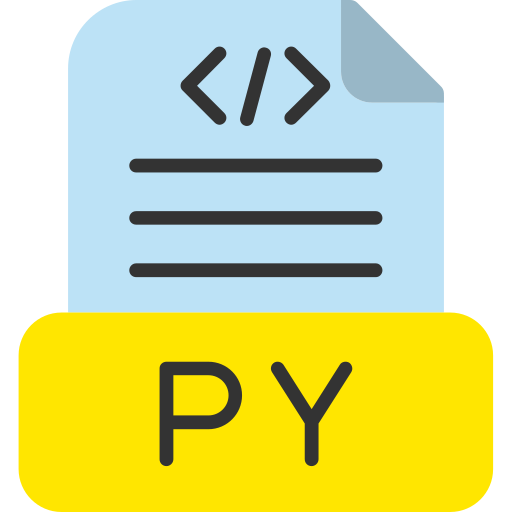
\includegraphics[width=30pt,keepaspectratio]{assets/py_code.png}};

% AST Graph
\node[v1,label=above:$V1$,right=40pt of code,yshift=-15pt] (v1) {};
\node[v2,label=above:$V2$,above right=20pt and 20pt of v1] (v2) {};
\node[v3,label=above:$V3$,right=40pt of v1] (v3) {};
\node[v4,label=above:$V4$,above right=20pt and 20pt of v3] (v4) {};

\path[e1] (v1) -- (v2);
\path[e2] (v2) -- (v4);
\path[e3] (v3) -- (v2);
\path[e4] (v4) -- (v3);

\node[fit=(v1) (v2) (v3) (v4),label={[font=\small]below:AST Graph}] (graph) {};

\path[arrow] (code) -- (graph);

% Identifiers
\node[identifier,above right=30pt and 12pt of v4] (ti) {Type\\Identifiers};

\node[vi,right=25pt of ti,label={[font=\small]below:[node]}] (v) {v};
\node[ei,right=10pt of v,label={[font=\small]below:[edge]}] (e) {e};

\node[below=10pt of ti,identifier] (ni) {Node\\Identifiers};

\node[v1,rounded,right=5pt of ni] (n1) {1};
\node[v2,rounded,right=5pt of n1] (n2) {2};
\node[v3,rounded,right=5pt of n2] (n3) {3};
\node[v4,rounded,right=5pt of n3] (n4) {4};

\path[draw,decorate,decoration={brace,mirror,amplitude=5pt,raise=2pt}] (n1.south) -- (n4.south) node[midway,below=5pt,font=\small] (orthnormal) {orthonormal};

    {[on background layer]
\node[fit=(ti) (ni) (v) (e) (n1) (n2) (n3) (n4) (orthnormal),fill=Gray!20,above right=-20pt and 10pt of v4,minimum size=60pt,rounded corners=4pt] (identifiers) {};
}

\path[dashed arrow] (graph) |- (identifiers);

\path[draw,->,black] (n4)+(15pt,0) -- +(35pt,0);
\path[draw,->,black] (e)+(33pt,0) -- +(53pt,0);

% V1

\node[v1,rounded,right=40pt of n4.north,yshift=0.5pt] (nt1-1) {1};
\node[v1,rounded,below=1pt of nt1-1] (nt1-2) {1};

    {[on background layer]
\node[fit=(nt1-1) (nt1-2),rounded corners=4pt,rectangle,draw=black] (nt1) {};
}

\node[vi,above=10pt of nt1-1] (vi-1) {v};

\node[v1,below=27pt of nt1-1] (v1-1) {};

\path[draw,->,black] (graph.center)+(35pt,-5pt) -- (332pt,-5pt) node[midway,below=5pt,font=\small] (mask) {Randomly masked type annotations};

    {[on background layer]
\path[draw,->,black] (v1-1) -- +(0,95pt);
}

% E1

\node[v1,rounded,right=10pt of nt1-1] (nt2-1) {1};
\node[v2,rounded,below=1pt of nt2-1] (nt2-2) {2};

    {[on background layer]
\node[fit=(nt2-1) (nt2-2),rounded corners=4pt,rectangle,draw=black] (nt2) {};
}

\node[ei,above=10pt of nt2-1] (ei-1) {e};

\node[below=27pt of nt2-1,opacity=0.0,minimum size=16pt,rectangle] (e1-1-tmp) {};
\node[fill=Emerald,below=27pt of nt2-1,node distance=10pt,minimum width=4pt,minimum height=16pt,rectangle,inner sep=0,rotate around={135:(e1-1-tmp.center)}] (e1-1) {};

    {[on background layer]
\path[draw,->,black] (e1-1) -- +(0,95pt);
}

% V2

\node[v2,rounded,right=10pt of nt2-1] (nt3-1) {2};
\node[v2,rounded,below=1pt of nt3-1] (nt3-2) {2};

    {[on background layer]
\node[fit=(nt3-1) (nt3-2),rounded corners=4pt,rectangle,draw=black] (nt3) {};
}

\node[vi,above=10pt of nt3-1] (vi-2) {v};

\node[v2,semicircle,minimum size=8pt,below=30.5pt of nt3-1,node distance=10pt] (v2-1) {};

    {[on background layer]
\path[draw,->,black] (v2-1) -- +(0,95pt);
}

% E2

\node[v2,rounded,right=10pt of nt3-1] (nt4-1) {2};
\node[v3,rounded,below=1pt of nt4-1] (nt4-2) {3};

    {[on background layer]
\node[fit=(nt4-1) (nt4-2),rounded corners=4pt,rectangle,draw=black] (nt4) {};
}

\node[ei,above=10pt of nt4-1] (ei-2) {e};

\node[below=27pt of nt4-1,opacity=0.0,minimum size=16pt,rectangle] (e2-1-tmp) {};
\node[fill=SpringGreen!50,below=27pt of nt4-1,node distance=10pt,minimum width=4pt,minimum height=16pt,rectangle,inner sep=0,rotate around={45:(e2-1-tmp.center)}] (e2-1) {};

    {[on background layer]
\path[draw,->,black] (e2-1) -- +(0,95pt);
}

% V3

\node[v3,rounded,right=10pt of nt4-1] (nt5-1) {3};
\node[v3,rounded,below=1pt of nt5-1] (nt5-2) {3};

    {[on background layer]
\node[fit=(nt5-1) (nt5-2),rounded corners=4pt,rectangle,draw=black] (nt5) {};
}

\node[vi,above=10pt of nt5-1] (vi-3) {v};

\node[v3,semicircle,minimum size=8pt,below=30.5pt of nt5-1,node distance=10pt] (v3-1) {};

    {[on background layer]
\path[draw,->,black] (v3-1) -- +(0,95pt);
}

% E3

\node[v3,rounded,right=10pt of nt5-1] (nt6-1) {3};
\node[v4,rounded,below=1pt of nt6-1] (nt6-2) {4};

    {[on background layer]
\node[fit=(nt6-1) (nt6-2),rounded corners=4pt,rectangle,draw=black] (nt6) {};
}

\node[ei,above=10pt of nt6-1] (ei-3) {e};

\node[below=27pt of nt6-1,opacity=0.0,minimum size=16pt,rectangle] (e3-1-tmp) {};
\node[fill=Emerald!50,below=27pt of nt6-1,node distance=10pt,minimum width=4pt,minimum height=16pt,rectangle,inner sep=0,rotate around={135:(e3-1-tmp.center)}] (e3-1) {};

    {[on background layer]
\path[draw,->,black] (e3-1) -- +(0,95pt);
}

% V4

\node[v4,rounded,right=10pt of nt6-1] (nt7-1) {4};
\node[v4,rounded,below=1pt of nt7-1] (nt7-2) {4};

    {[on background layer]
\node[fit=(nt7-1) (nt7-2),rounded corners=4pt,rectangle,draw=black] (nt7) {};
}

\node[vi,above=10pt of nt7-1] (vi-4) {v};

\node[v4,below=27pt of nt7-1,node distance=10pt] (v4-1) {};

    {[on background layer]
\path[draw,->,black] (v4-1) -- +(0,95pt);
}

% E3

\node[v4,rounded,right=10pt of nt7-1] (nt8-1) {4};
\node[v2,rounded,below=1pt of nt8-1] (nt8-2) {2};

    {[on background layer]
\node[fit=(nt8-1) (nt8-2),rounded corners=4pt,rectangle,draw=black] (nt8) {};
}

\node[ei,above=10pt of nt8-1] (ei-4) {e};

\node[below=27pt of nt8-1,opacity=0.0,minimum size=16pt,rectangle] (e4-1-tmp) {};
\node[fill=SpringGreen,below=27pt of nt8-1,node distance=10pt,minimum width=4pt,minimum height=16pt,rectangle,inner sep=0,rotate around={90:(e4-1-tmp.center)}] (e4-1) {};

    {[on background layer]
\path[draw,->,black] (e4-1) -- +(0,95pt);
}


\path (v2-1) -- (e3-1) node[identifier,midway,below=12pt] (embeddings) {Node and Edge Tokens\\with Token-wise Embedding};

% Transformer

\node[fit=(nt1-1) (nt1-2) (nt2-1) (nt2-2) (nt3-1) (nt3-2) (nt4-1) (nt4-2) (nt5-1) (nt5-2) (nt6-1) (nt6-2) (nt7-1) (nt7-2) (nt8-1) (nt8-2),fill=Gray!20,rounded,draw,label=center:Transformer Encoder + MLP,above=20pt of vi-1,anchor=south west,xshift=-12pt] (transformer) {};

% Prediction

\node[v2,above=80pt of vi-2] (vp-2) {};
\node[v3,above=80pt of vi-3] (vp-3) {};

\path[draw,->,*|,black,shorten >=2pt] (transformer.north) to (vp-2);

\path[draw,->,*|,black,shorten >=2pt] (transformer.north) to (vp-3);

\path (vp-2) -- (vp-3) node[identifier,midway,above=12pt] (embeddings) {Type annotation predictions};


\end{tikzpicture}}
    \caption{GraphTyper Architecture}
    \label{fig:model}
\end{figure*}

In our model we use node and edge types extracted from code as token features.
Node ground truth annotations are added to the features and randomly masked during training.
As loss, weighted cross entropy is used due to the imbalance of the dataset.
The overall architecture of the model is displayed at Figure~\ref{fig:model}.
We develop two types of Transformers: Masked Transformer Encoder-only Model and Masked Transformer Encoder-Decoder Model.

\subsubsection{Masked Transformer Encoder-only Model}

Predicting type annotations in graph domain is a node classification task.
However, since we are using a Pure Transformer with graphs represented as sequence of tokens, the task can be reduced to token classification.
In the Natural Language Processing (NLP) domain this is a very common task, also known as Named Entity Recognition (NER).

Encoder-only architecture has been widely used for the NER task, namely BERT is one of the most popular models~\cite{liu2021nerbert,Darji_2023}.
We adapt similar architecture by randomly masking type annotations.
We then apply a classifier head to the output of TokenGT~\cite{kim_pure_2022} to get logits of type annotations.

\subsubsection{Masked Transformer Encoder-Decoder Model}

In addition, we develop an Encoder-Decoder model architecture, inspired by GMAE~\cite{zhang2022graph}.
However, instead of masking the entire nodes as in the mentioned paper, we only mask features corresponding to type annotations
same as with Encoder-only Model.

Masked model architecture is very versatile and the pretrained model can be later easily fine-tuned for other tasks,
similar to the approaches from the NLP-domain~\cite{liu2021nerbert}.
For example, error~\cite{bieber2022static} and vulnerability~\cite{sun2023exploring} data can be added to the code graph to detect and fix them~\cite{nguyen_regvd_2021,li_vuldeepecker_2018,cao_bgnn4vd_2021,li_sysevr_2021,russell_automated_2018}.

\section{Experiments and Ablation Results}\label{sec:experiment-results-and-ablation}
To select the final model architecture, we test different models.
For our experiments and ablation analysis, we train and test the models using one sample repository.
We also limit the number of types in the vocabulary to one hundred to speed up training and use less resources.
To test the models, we calculate Top-n predictions similar to the previous work~\cite{mir_type4py_2021}.
Table~\ref{tab:ablation} depicts the results of the experiments and ablation.

\subsection{Validating the necessity of node and type identifiers that encode graph structure}\label{subsec:validating-the-necessity-of-node-and-type-identifiers-that-encode-graph-structure}

First of all, we remove the node and type identifiers introduced by Kim et. Al~\cite{kim_pure_2022} our ablation analysis demonstrates that indeed, the graph structure embeddings play a key role in model quality.
By removing them from the model, we are left with a simple Transformer that makes predictions only based on AST nodes and edges types without any information about graph structure.
Such a model outputs the worst results among all the experiments.

\subsection{Using the model without node type annotations}\label{subsec:using-the-model-without-node-type-annotations}

In addition, we try to remove the type annotations from the model completely.
This alteration turns our training into a masked NER task.
Surprisingly, our model performs well in such conditions.
This means that the selected graph representation of code contains a lot of necessary information to infer types.

\subsection{Increasing the number of parameters}\label{subsec:increasing-the-number-of-parameters}

As we can see, increasing the number of parameters also increases the predictive power of the model.
However, increasing the parameters indefinitely is not very practical and requires a lot of computational resources~\cite{arutyunov_big_2022}.
Therefore, we don't change the parameter number of the final model, so it remains compact.

\subsection{Testing different context length}\label{subsec:testing-different-context-length}

As for the context length, i.e., maximum number of nodes in graph (512 vs. 1024), our findings are aligned with the conclusions from previous work~\cite{arutyunov_big_2022}:
longer context increases the performance of the model.
However, the AST representation of source code is very bloated and even having a lot of nodes in the graph might not capture
enough useful information to make quality predictions.
In addition, increasing the context length drastically slows down the training process.
Thus, in future research, we will be working on finding a better and more compact graph representation of code.

\subsection{Testing different Transformer architectures}\label{subsec:testing-different-transformer-architectures-(encoder-only-vs-encoder-decoder)}

Recently, Masked Graph Autoencoders have been applied for the tasks of link prediction and node classification~\cite{tan2022mgae},
as well as feature reconstruction~\cite{zhang2022graph, hou2022graphmae}.
To validate the robustness of the Encoder-only Model, we also implement a Masked Autoencoder Model.
For this, we adapt the approach of Hou et. al~\cite{hou2022graphmae} for our model.
We introduce a learnable mask token and a decoder based on the encoder layers.
We reconstruct the type annotations by re-masking the target nodes before feeding them into the decoder.
However, we do not observe as good results as with a simple Encoder-only model.

\begin{table}
    \centering
    \caption{Expirement results of Top-n predictions for different model variants.}
    \label{tab:ablation}
    \begin{tabular}{llrrrr}
\toprule
 & \% Match & \multicolumn{2}{r}{Exact} & \multicolumn{2}{r}{Up to Parametric Type} \\
 & Context Length & 512 & 1024 & 512 & 1024 \\
Model & Top-n &  &  &  &  \\
\midrule
\multirow[t]{4}{*}{Base (51 mln)} & Top-1 & 30.88 & 31.12 & 36.55 & 35.83 \\
 & Top-3 & 40.33 & 42.79 & 50.37 & 56.30 \\
 & Top-5 & 42.82 & 45.30 & 56.01 & 60.12 \\
 & Top-10 & 48.03 & 48.72 & 64.98 & 64.59 \\
\cline{1-6}
\multirow[t]{4}{*}{Ablated (51 mln)} & Top-1 & 10.15 & 21.39 & 19.46 & 31.09 \\
 & Top-3 & 15.06 & 38.94 & 29.40 & 54.08 \\
 & Top-5 & 16.81 & 41.19 & 37.91 & 56.97 \\
 & Top-10 & 22.97 & 46.27 & 46.72 & 62.05 \\
\cline{1-6}
\multirow[t]{4}{*}{Deep (214 mln)} & Top-1 & 26.69 & 32.93 & 29.93 & 37.95 \\
 & Top-3 & 40.15 & 44.07 & 48.82 & 53.55 \\
 & Top-5 & 44.18 & 46.23 & 57.11 & 60.36 \\
 & Top-10 & 49.49 & 52.69 & 67.77 & 69.63 \\
\cline{1-6}
\multirow[t]{4}{*}{Big (331 mln)} & Top-1 & 30.90 & 32.77 & 33.59 & 38.29 \\
 & Top-3 & 42.75 & 43.36 & 49.62 & 51.46 \\
 & Top-5 & 47.28 & 45.21 & 58.25 & 55.92 \\
 & Top-10 & 52.72 & 50.25 & 68.53 & 66.20 \\
\cline{1-6}
\multirow[t]{4}{*}{Final (432 mln)} & Top-1 & 29.25 & 34.71 & 36.97 & 36.43 \\
 & Top-3 & 39.93 & 45.47 & 53.19 & 55.02 \\
 & Top-5 & 46.58 & 50.70 & 63.29 & 64.58 \\
 & Top-10 & 54.21 & 57.60 & 72.30 & 72.15 \\
\cline{1-6}
\bottomrule
\end{tabular}


\end{table}

\section{Known Limitations}\label{sec:known-limitations}
\subsection{Size of Type Vocabulary}\label{subsec:size-of-type-vocabulary}

Since we define our task as node (token) classification, we feed our transformer output into a classifier linear head.
Therefore, our type vocabulary is limited.
Because of the computational resources constraints, we limit it to one thousand types.

This issue is addressable by formulating the task as Deep Similarity Learning Problem~\cite{chopra2005learning,liao2018tripletbased}.
In this way, the model will output vector representations of types that can be grouped into cluster of similar types.
After that, an algorithm such as KNN~\cite{knn} is used to transform vector representation into a probability of each type~\cite{allamanis2020typilus,mir_type4py_2021}.

\subsection{Absence of Natural Language information}\label{subsec:absence-of-natural-language-information}

In our work, we use only categorical features of nodes and edges of code graph, e.g. AST node types and Python type annotations.
Therefore, it would be challenging to apply it directly for tasks such as code generation,
because the representation doesn't encode any information about variable names.

There are several approaches that would help address this issue.
Firstly, it is possible to use the model output as graph encoding that would be later fed into another model along with tokenized code~\cite{tipirneni_structcoder_2022}.
This approach could also address the issue from the previous Section~\ref{subsec:size-of-type-vocabulary}, since types would be treated as a set of text tokens~\cite{peng2023generative}.
Secondly, it is possible to use neural networks to infer variables' names from the context they are used in~\cite{bavishi2018context2name}.


\section{Future Work}\label{sec:future-work}
In this work, we explored the application of Graph Transformers for type inference.
The versatile architecture of the proposed solution lets us explore other tasks.

\subsection{Universal code graph representation}\label{subsec:universal-code-graph-representation}

If a universal version of graph code representation is used, similar to CPG~\cite{yamaguchi2014modeling},
we can train the model for multiple programming languages~\cite{wang_unified_2022}.
However, because of the differences of type systems, separate models would be trained for each programming language for better results.

\subsection{Detecting duplicates}\label{subsec:detecting-duplicates}

It is crucial to address the issue of duplicates in source code to train neural networks for code~\cite{allamanis2020typilus,mir_type4py_2021}.
Several architectures have already been used for such task: Transformers~\cite{zhang2023efficient}, GNNs~\cite{wang_detecting_2020} and RNNs~\cite{yasaswi2017plagiarism}.
We believe that the graph representation obtained with our model can be successfully used for code clone detection.

\subsection{Code and docstring generation}\label{subsec:code-generation}

Firstly, we can train the model using a technique similar to generative pretrained models~\cite{radford_language_2019,brown_language_2020} or masked language models~\cite{tipirneni_structcoder_2022} to generate code.
Secondly, our model can be used to generate code summarization or docstring generation~\cite{barone_parallel_2017,liu_haconvgnn_2021}.
This could only be possible if we adapt some of the approach discussed in the previous Section~\ref{subsec:absence-of-natural-language-information}

\subsection{Vulnerability and error detection}\label{subsec:vulnerability-and-error-detection}

Another useful task is to detect errors and generate fixes~\cite{bhatia_automated_2016,marginean_sapfix_2019}.
This is possible by simply adding features that contain error indication or types.
Similar approach can be used to scan for vulnerabilities~\cite{li_vuldeepecker_2018,russell_automated_2018,nguyen_regvd_2021}.
Fixing bugs and vulnerabilities, however, would imply that the graph structure could change.
Therefore, solving this task would require the model to be modified for graph generation~\cite{khajenezhad2022gransformer}.

\subsection{Refactoring}\label{subsec:refactoring}

Finally, we can extend our model with information about changes to analyze them and propose refactoring possibilities~\cite{cabrera_lozoya_commit2vec_2021}.
This goal could be achieved by using the model from the previous Section~\ref{subsec:vulnerability-and-error-detection}.

\section{Conclusion}\label{sec:conclusion}

As for the conclusion, we were able to create a universal model based on TokenGT~\cite{kim_pure_2022} and code represented as graphs.
One of the most important advantages of this model is that it uses the code graph directly.
Secondly, the model can be modified to fit other tasks, such as code generation and summarization, docstring generation, refactoring and many more.
The code graph can also be extended by different features and node types, since the representation does not differ depending on graph structure.

\section{Acknowledgments}\label{sec:acknowledgments}

This research was supported in part through computational resources of HPC facilities at HSE University~\cite{kostenetskiy_hpc_2021}.

\printbibliography

\end{document}